\documentclass[a4paper,11pt]{article}
\usepackage[a4paper,right=1.5cm,top=1.5 cm]{geometry} %margenes en A4
%\usepackage[spanish]{babel} %idioma principal
\sloppy %suaviza las reglas de ruptura de líneas de LaTeX
%%%%%%%%%%%%%%%%%%%%%%%%%%%%PAQUETESNECESARIOS
\usepackage{latexsym} % Símbolos
%\usepackage[linktocpage]{hyperref}%hipervinculos 
%\usepackage[dvips]{graphicx}
\usepackage[pdftex]{graphicx}

%\usepackage{graphicx}
%\usepackage{caption}
\usepackage{subcaption}

\usepackage{multicol}
\usepackage{multirow}
%\usepackage{subfig}
\usepackage{longtable}
%\usepackage{eepic}
\usepackage{lscape}
\usepackage{array}
\usepackage{amssymb}
\usepackage{amsmath}
\usepackage{amsthm}
\usepackage[T1]{fontenc}
\usepackage{titlesec}
\usepackage[justification=centering]{caption}
\usepackage{titlepic}
\usepackage{listings} %algoritmos
%\usepackage[center, small]{caption2} %rótulos de imagenes y tablas 
%%%%%%%%%%%%%%%%%%%%%%%%%%%%PERSONALIZACIÓNDECABECERAS
%\pagestyle{myheadings}
\usepackage[utf8]{inputenc} %tildes
\usepackage{titlesec}
\usepackage[spanish]{babel}
%%%%%%%%%%%%%%%%%%%%%%%%%%%%%%%%%%%%%%COLORES%%%%%%%%%%%%%%%%%%%%%%%%%%%%%%%%%%%%%%%%%%%%%%%
%\usepackage[pdftex]{color}
%\usepackage[pdftex,colorlinks=true,linkcolor=blue,citecolor=green,urlcolor=blue]{hyperref}
%\phantomsection
%\renewcommand{\labelitemi}{$\bullet$}
\usepackage{hyperref}
%%%%%%%%%%%%%%%%%%%%%%%%%%%%%%%%%%%%%%%%%SIMBOLOSABREVIADOS%%%%%%%%%%%%%%%%%%%%%%%%%%%%%%%
\newcommand{\dd}{\mathrm{d}}
\newcommand{\dst}{\displaystyle}
\newcommand{\angstrom}{\mbox{\normalfont\AA}}
%\parindent=5mm
\parindent=0mm

\title{{\bf\Large Parcial 2}}
\author{\normalfont
\author[{Juan Sebastián Valbuena Bermúdez}\\\normalfont\sc Universidad Nacional de Colombia \\\normalfont\sc Electrodinámica 2}
\date{8 de noviembre de 2016}
\renewcommand\abstractname{Resumen}
\renewcommand\tablename{Tabla}
\renewcommand\figurename{Figura}
\renewcommand\refname{Referencias}
%\renewcomand\refname{date}

\begin{document}%

\maketitle
\author{}

\section*{Punto 1}
Sea una lámina plana de espesor $d$ cuya permitividad se corresponde con el modelo de plasma para altas frecuencias $(\omega >> \omega_o,\ \omega>>\Gamma)$, es decir,  $\epsilon(\omega)=\epsilon_0 (1- \omega_p^2 / \omega^2$. Dicha lámina está rodeada de vacío. Considere la incidencia de ondas planas que están linealmente polarizadas.


\subsection*{1.a}
Escriba la matriz de transferencia de la estructura tomando como planos de referencia dos planos situados por fuera de la lámina pero a una distancia infinitesimal de esta, es decir, en $z=0^-$ y $z=d^+$.

\textbf{Solución}

Se divide el espacio en tres regiones: 
\begin{itemize}
    \item Región 1: $z<0$, con permitividad $\epsilon = \epsilon_0$
    
    \item Región 2: $0<z<d$, con permitividad $\epsilon = \epsilon(\omega)$
    
    \item Región 3: $d<z$, con permitividad $\epsilon = \epsilon_0$
\end{itemize}

La matiz de transferencia $T$ se puede escribir como el producto de tres matrices:

$$T=T_{12}T_{2}T_{23}$$

donde $T_12$ es la matriz de tranferencia correspondiente a la interfaz entre las regiones



\[
\begin{bmatrix}
    x_{11}       & x_{12} & x_{13} & \dots & x_{1n} \\
    x_{21}       & x_{22} & x_{23} & \dots & x_{2n} \\
    \hdotsfor{5} \\
    x_{d1}       & x_{d2} & x_{d3} & \dots & x_{dn}
\end{bmatrix}
=
\begin{bmatrix}
    E_{11} & E_{12} & x_{13} & \dots  & x_{1n} \\
    E_{21} & E_{22} & x_{23} & \dots  & x_{2n} \\
    \vdots & \vdots & \vdots & \ddots & \vdots \\
    x_{d1} & x_{d2} & x_{d3} & \dots  & x_{dn}
\end{bmatrix}
\]
\subsection*{1.b}
r
\begin{figure}
    %\centering
    \begin{subfigure}[b]{0.48\textwidth}
        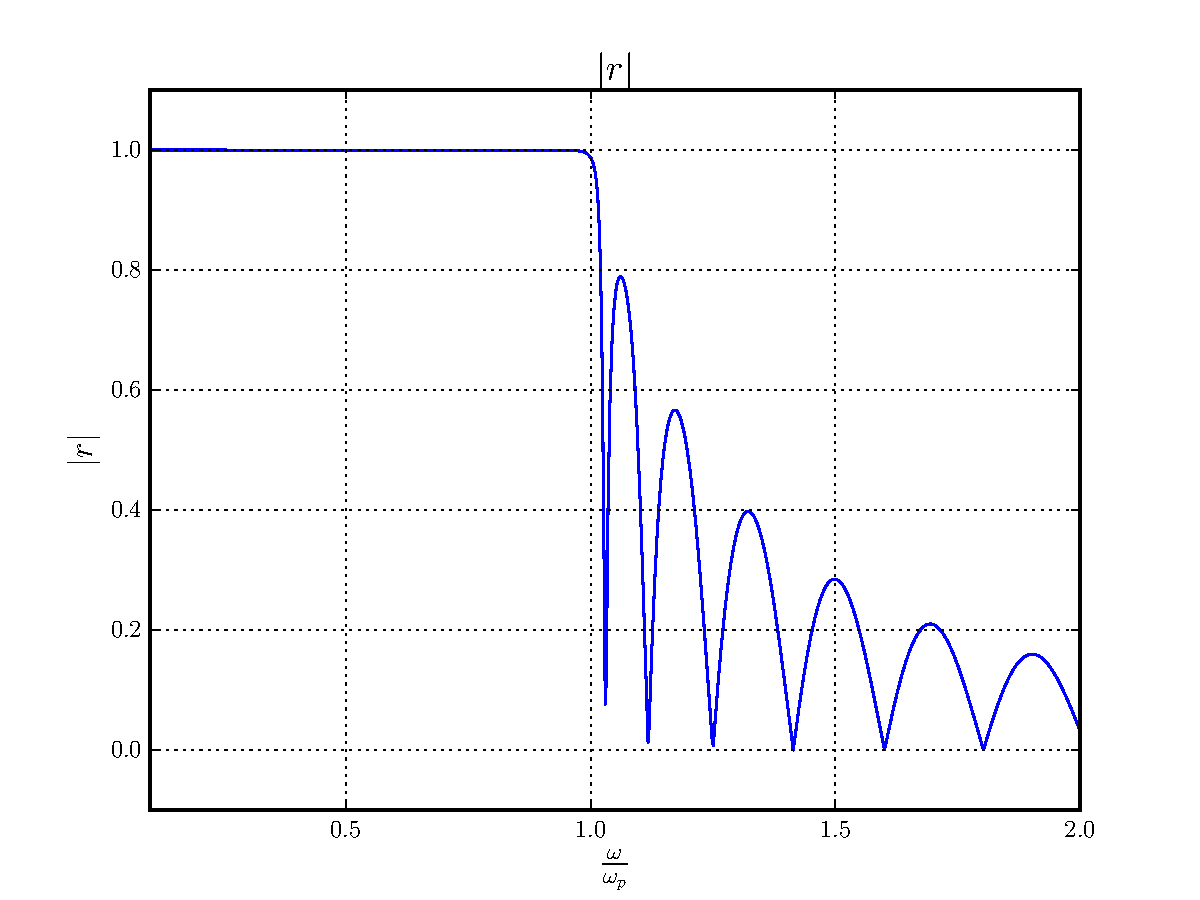
\includegraphics[width=\textwidth]{Punto1BC/r_N.pdf}
    \end{subfigure}
    \begin{subfigure}[b]{0.48\textwidth}
        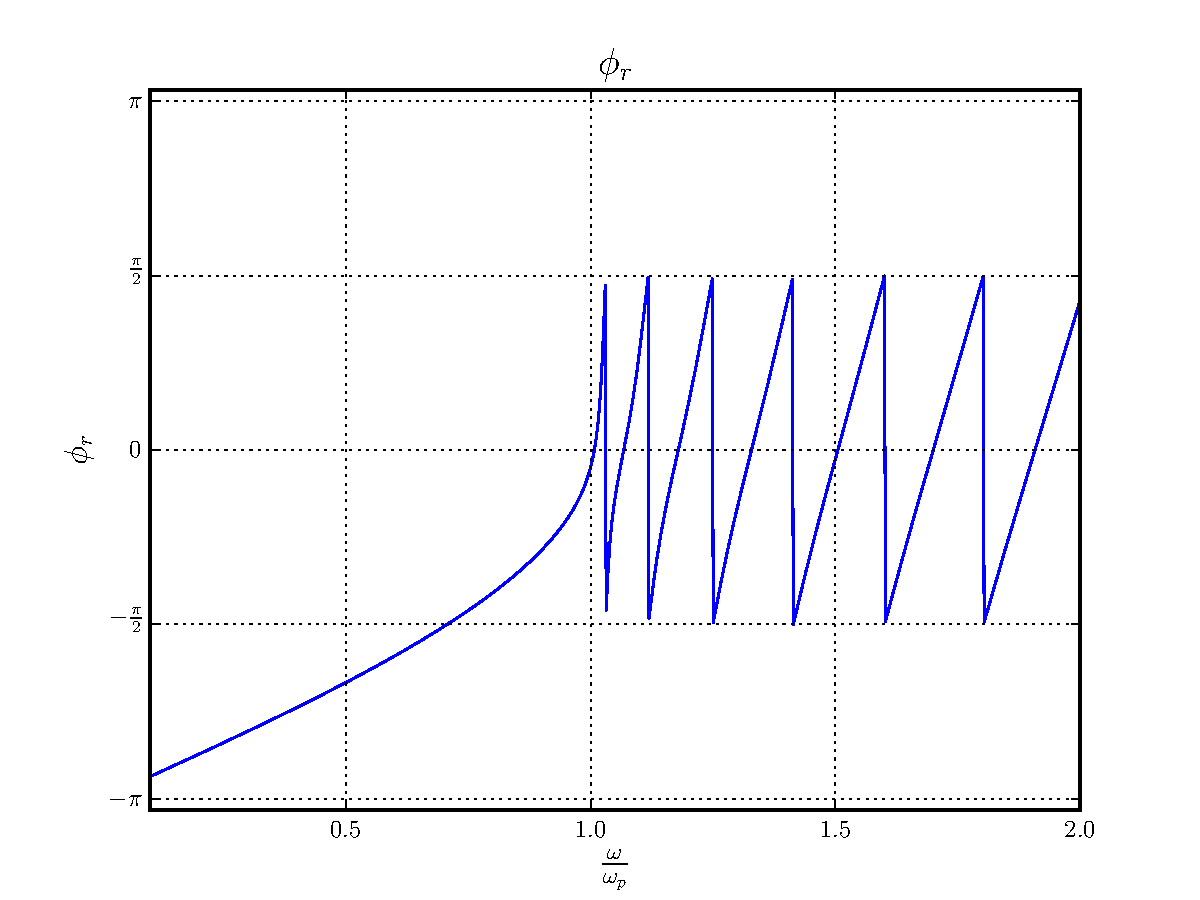
\includegraphics[width=\textwidth]{Punto1BC/r_f.pdf}
    \end{subfigure}
    \caption{Coefiecnte r}\label{r}
\end{figure}

t
\begin{figure}
    %\centering
    \begin{subfigure}[b]{0.48\textwidth}
        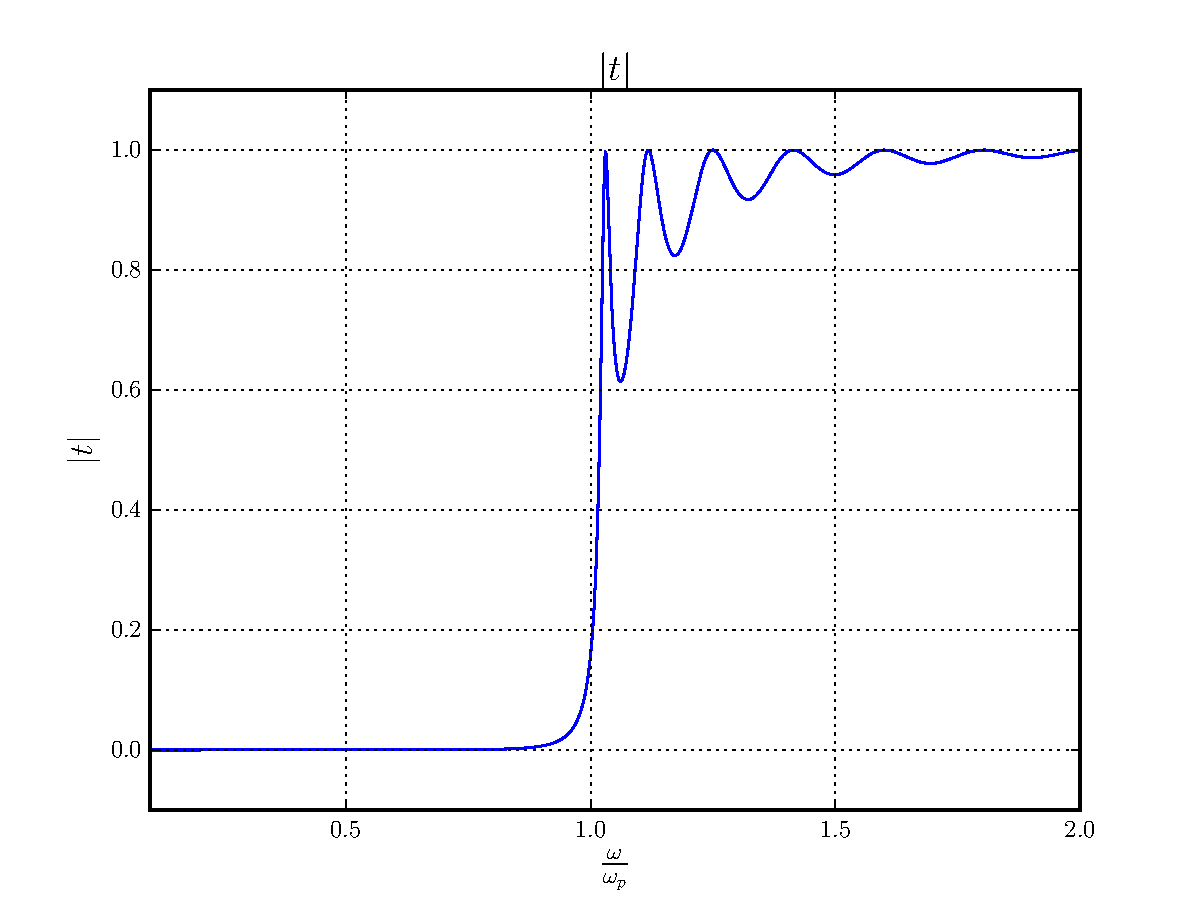
\includegraphics[width=\textwidth]{Punto1BC/t_N.pdf}
    \end{subfigure}
    \begin{subfigure}[b]{0.48\textwidth}
        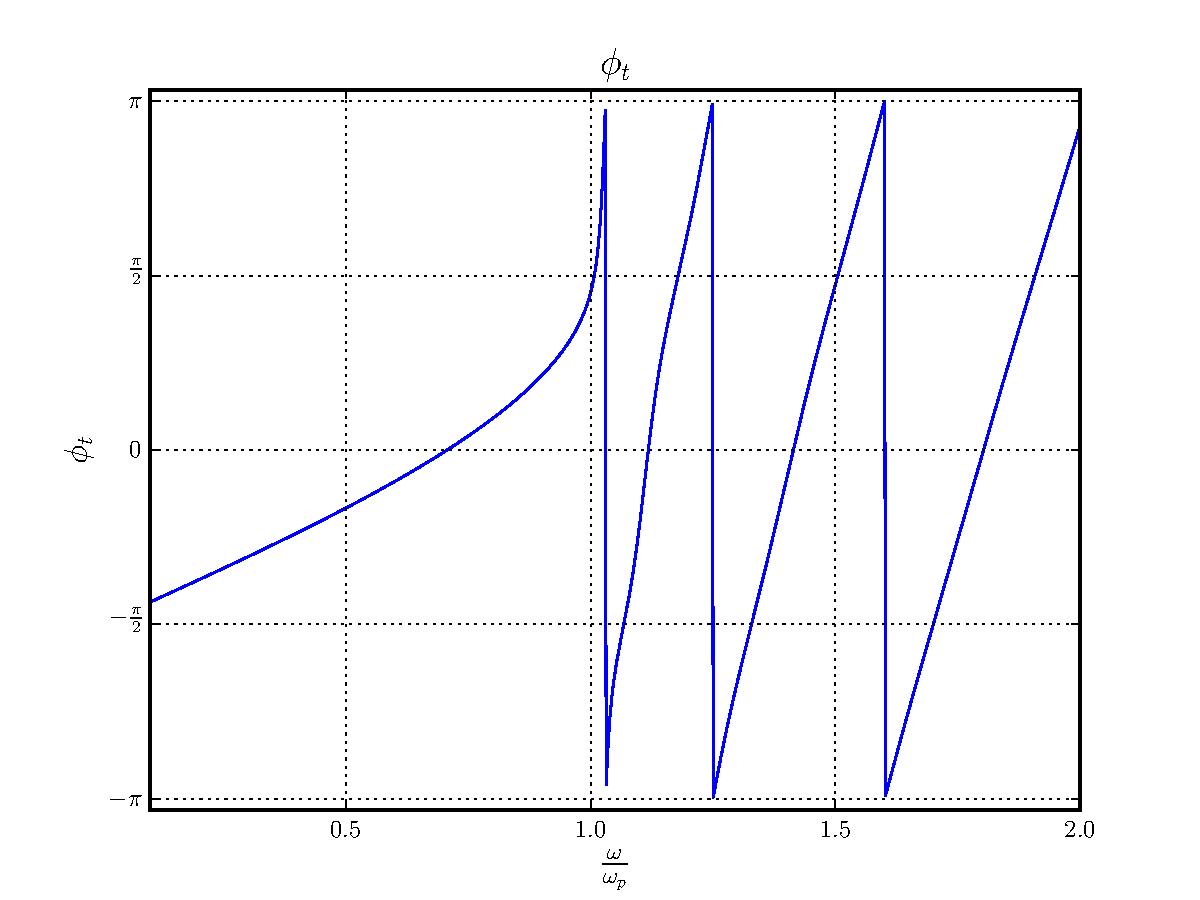
\includegraphics[width=\textwidth]{Punto1BC/t_f.pdf}
    \end{subfigure}
    \caption{Coefiecnte t}\label{t}
\end{figure}
\subsection*{1.c}  
  %FIGURA
                            \begin{figure}[!ht]
                            \centering 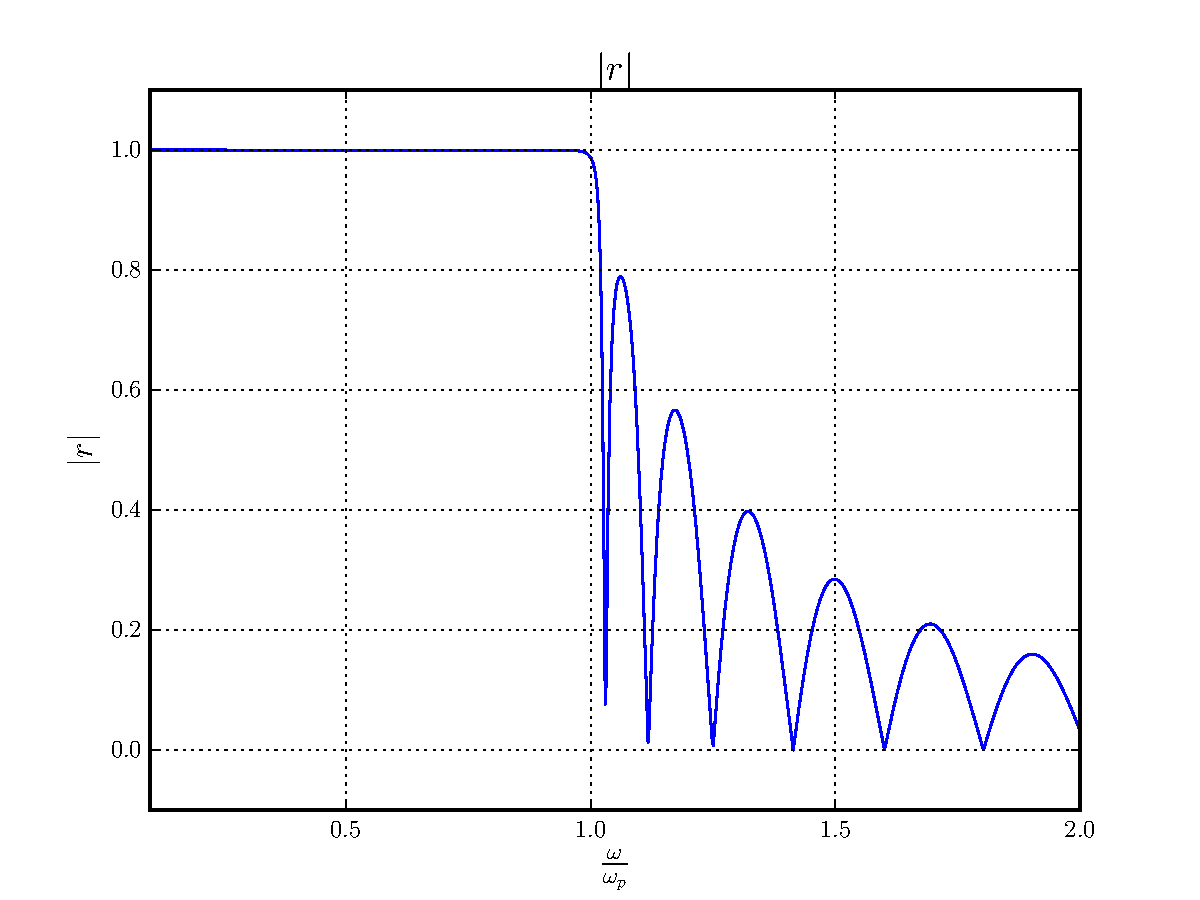
\includegraphics[width=0.9\textwidth]{Punto1BC/r_N.pdf}
                            \end{figure}
                            %FIGURA
                            %FIGURA
                            \begin{figure}[!ht]
                            \centering 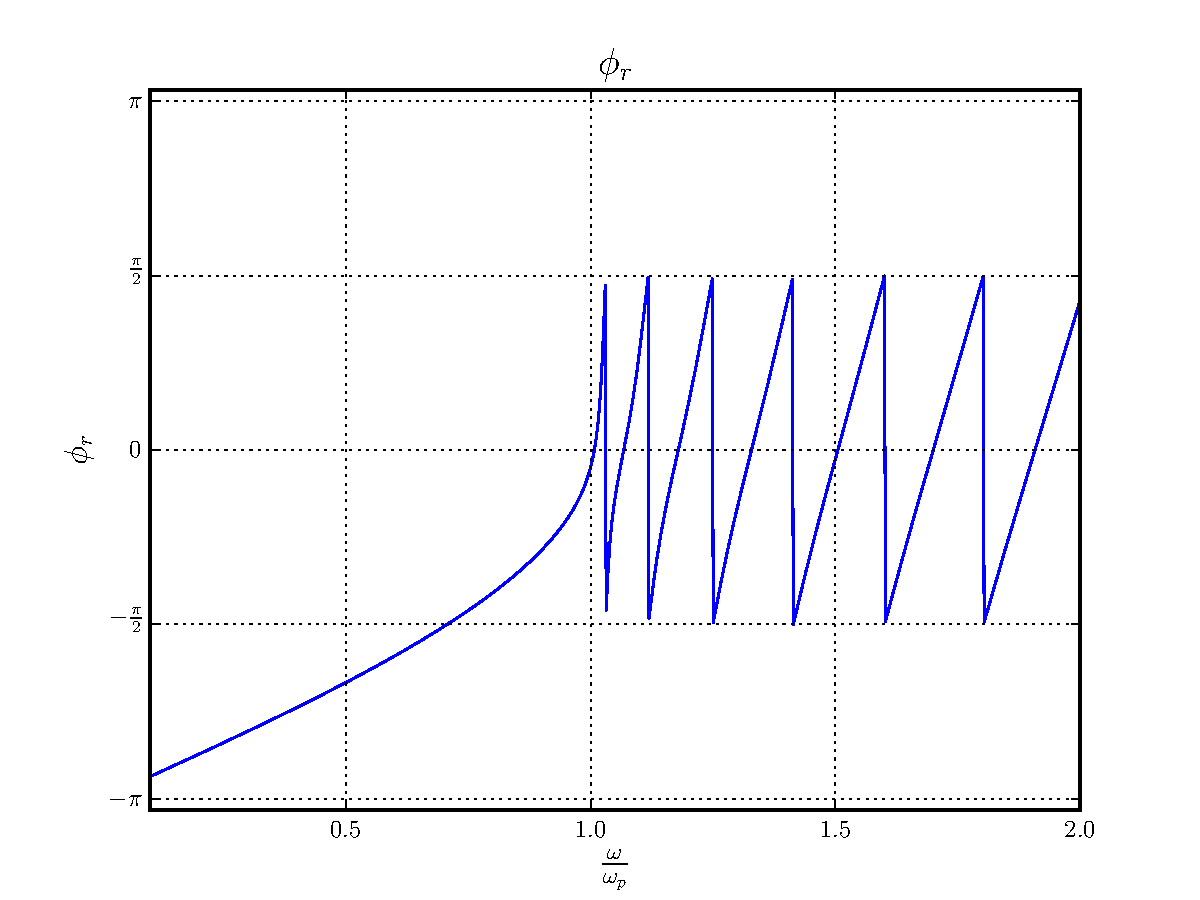
\includegraphics[width=0.9\textwidth]{Punto1BC/r_f.pdf}
                            \end{figure}
                            %FIGURA


                            %FIGURA
                            \begin{figure}[!ht]
                            \centering 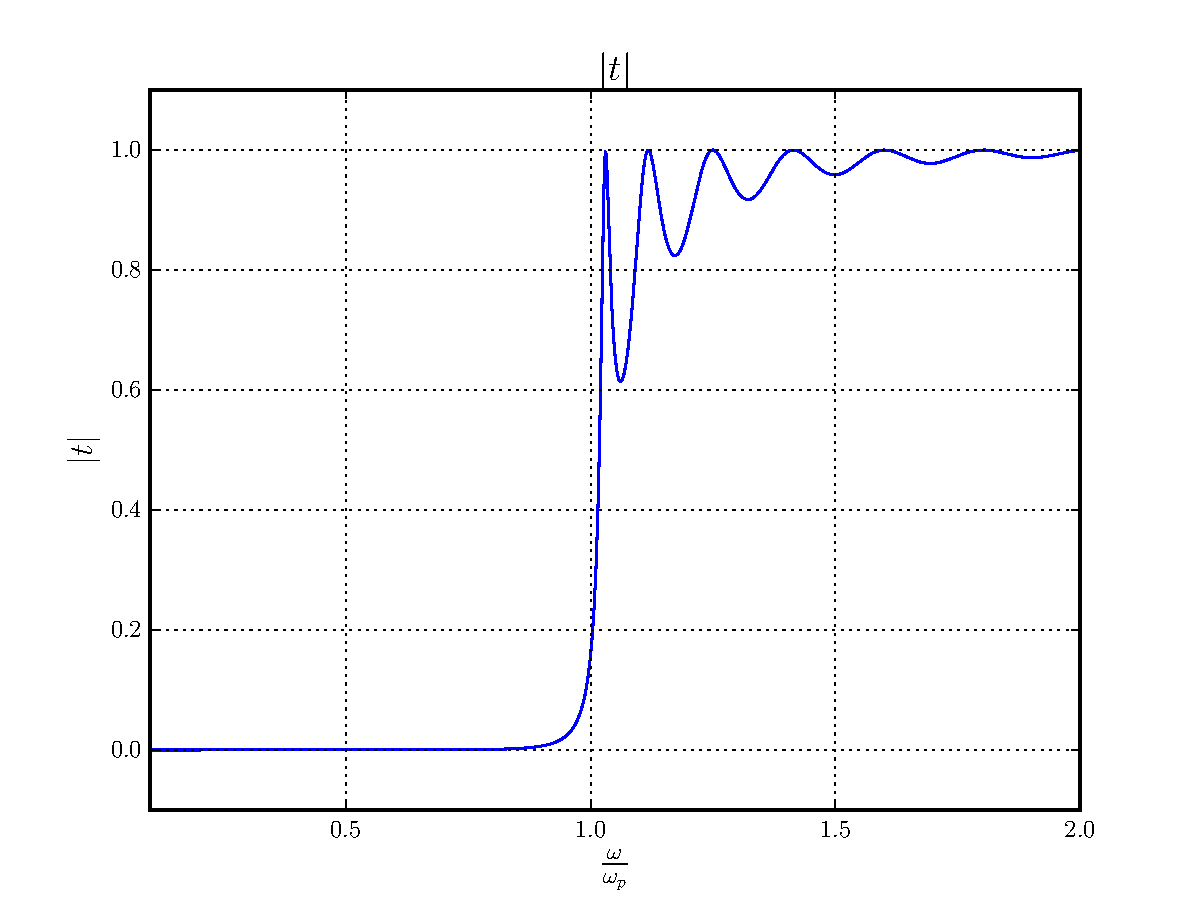
\includegraphics[width=0.9\textwidth]{Punto1BC/t_N.pdf}
                            \end{figure}
                            %FIGURA
                            %FIGURA
                            \begin{figure}[!ht]
                            \centering 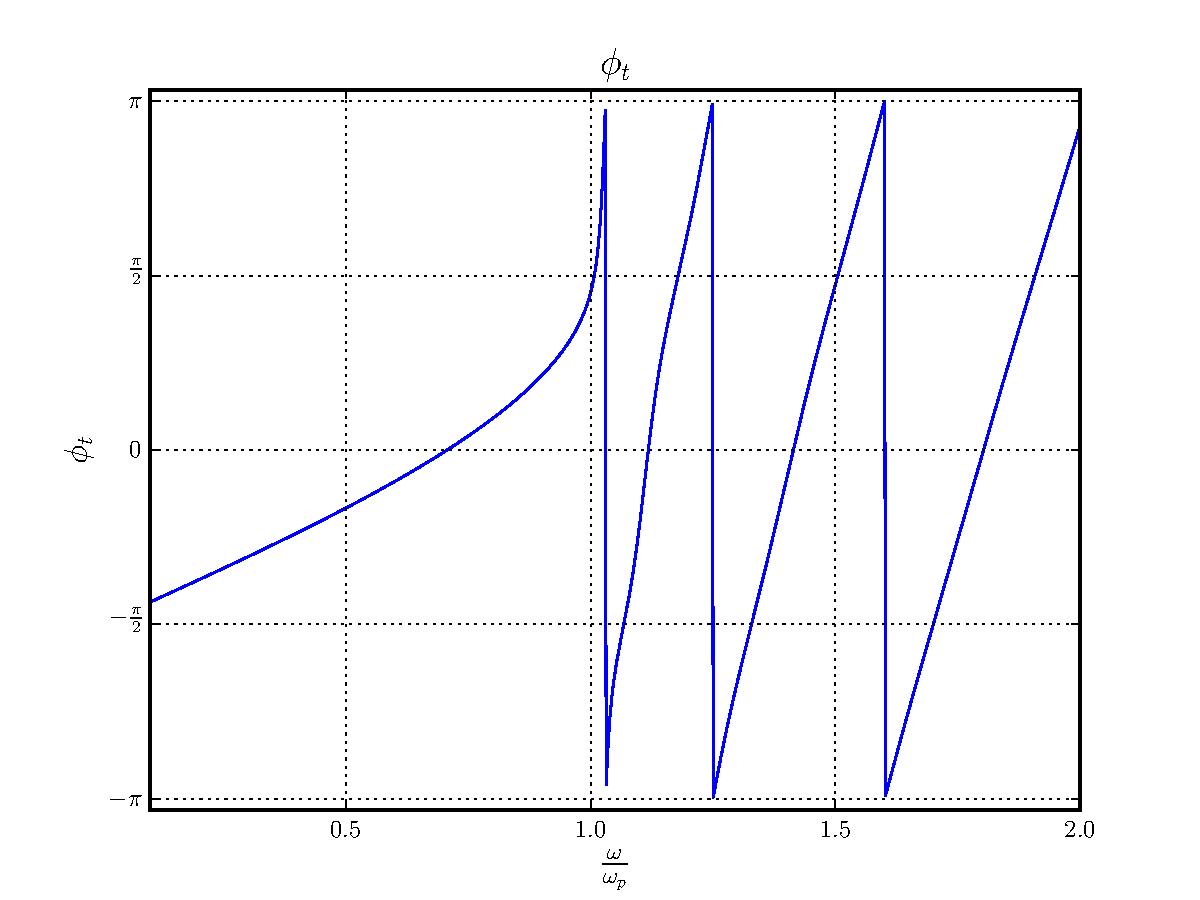
\includegraphics[width=0.9\textwidth]{Punto1BC/t_f.pdf}
                            \end{figure}
                            %FIGURA
Confirmación de $R+T=1$

                            %FIGURA
                            \begin{figure}[!ht]
                            \centering 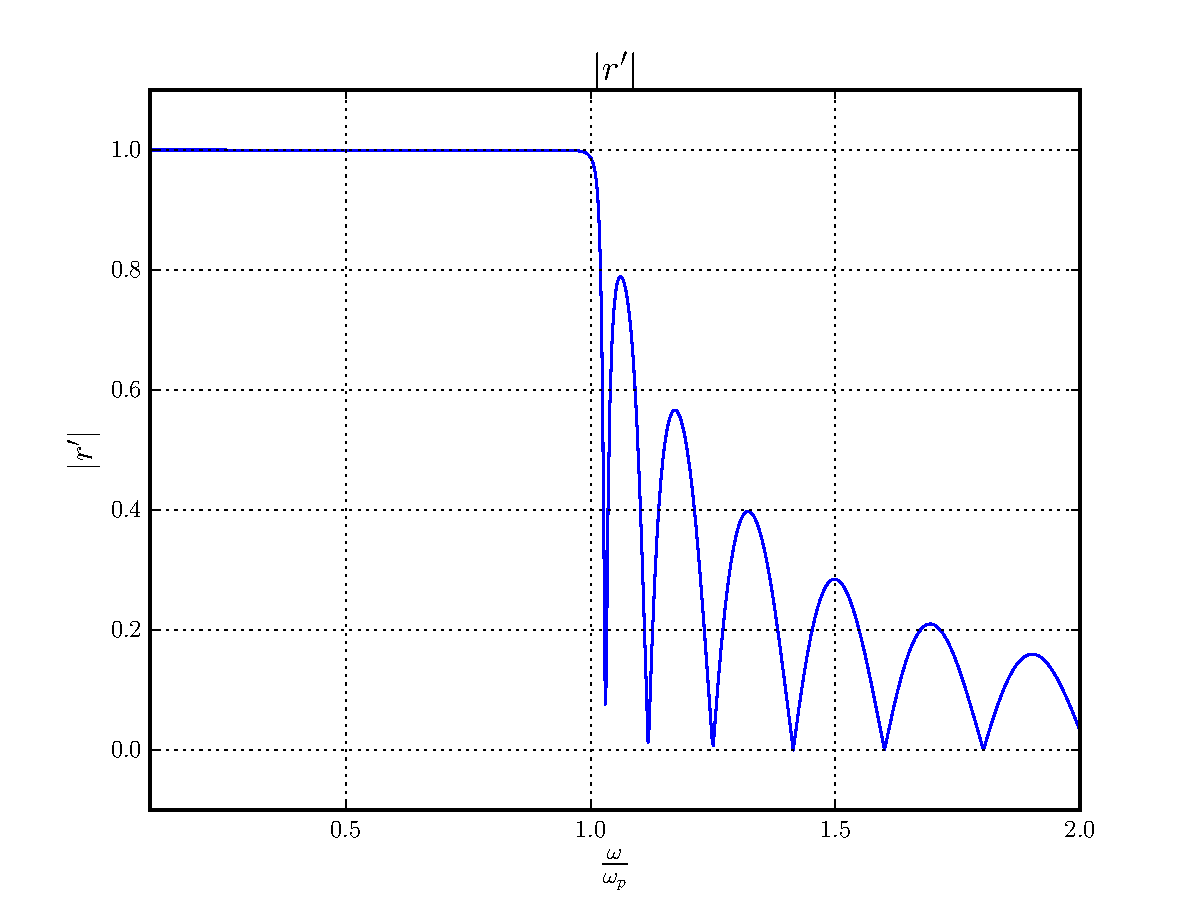
\includegraphics[width=0.9\textwidth]{Punto1BC/rp_N.pdf}
                            \end{figure}
                            %FIGURA
                            
                            %FIGURA
                            \begin{figure}[!ht]
                            \centering 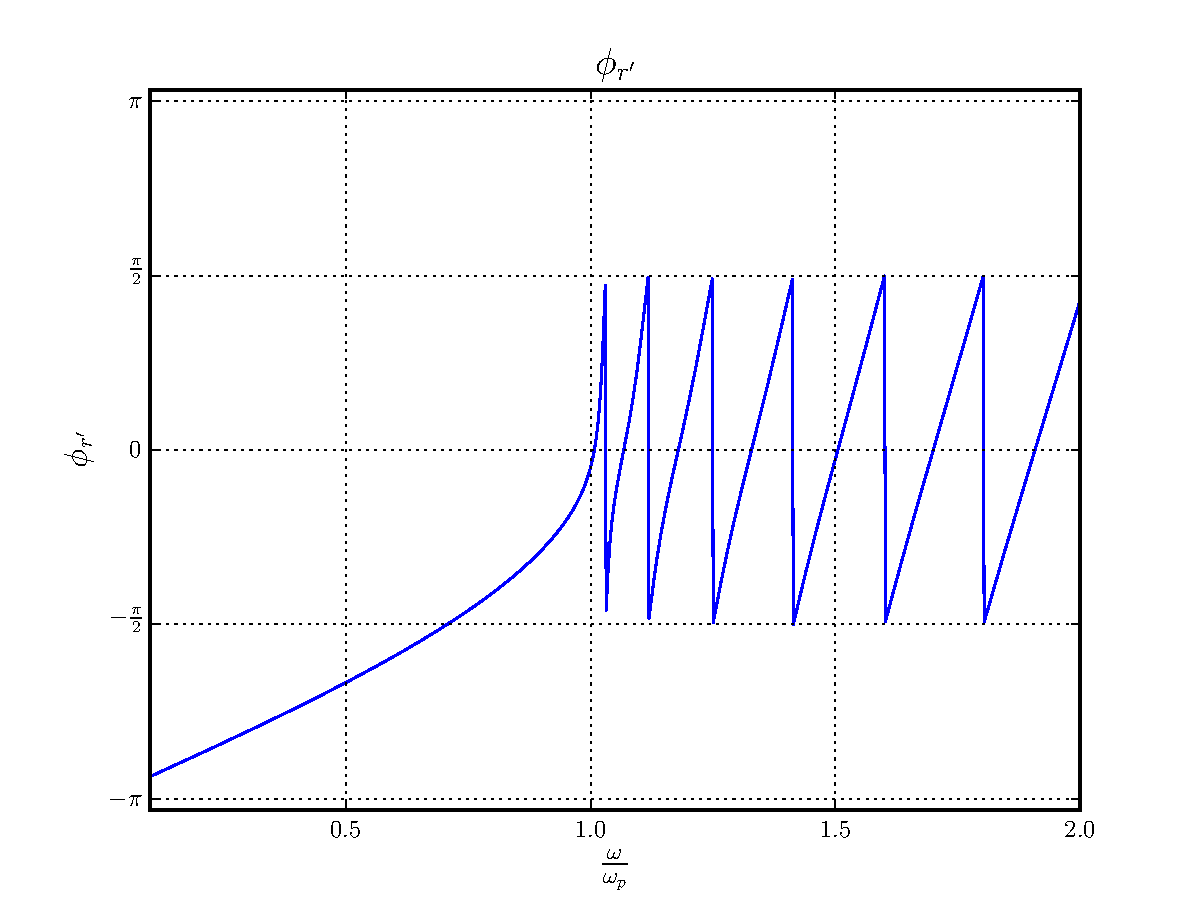
\includegraphics[width=0.9\textwidth]{Punto1BC/rp_f.pdf}
                            \end{figure}
                            %FIGURA


                            %FIGURA
                            \begin{figure}[!ht]
                            \centering 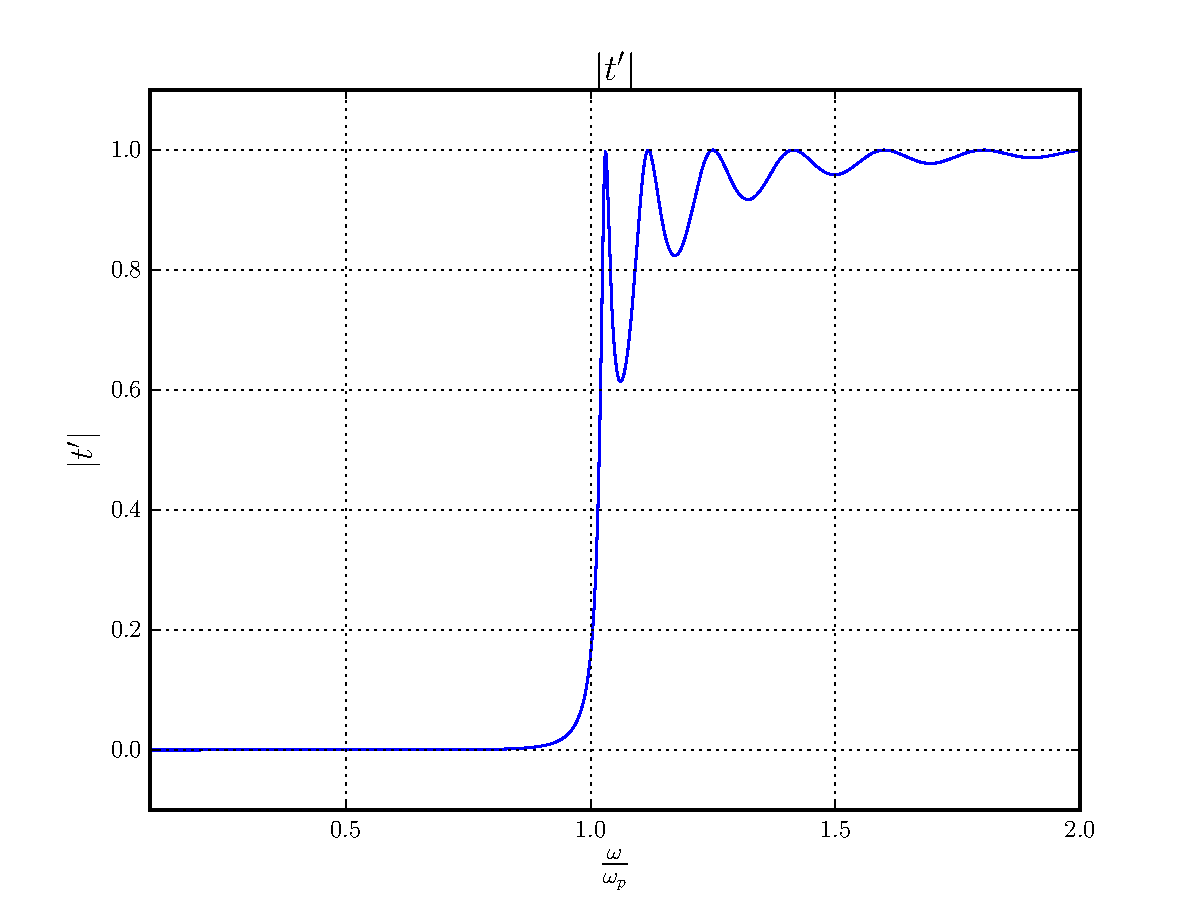
\includegraphics[width=0.9\textwidth]{Punto1BC/tp_N.pdf}
                            \end{figure}
                            %FIGURA
                            %FIGURA
                            \begin{figure}[!ht]
                            \centering 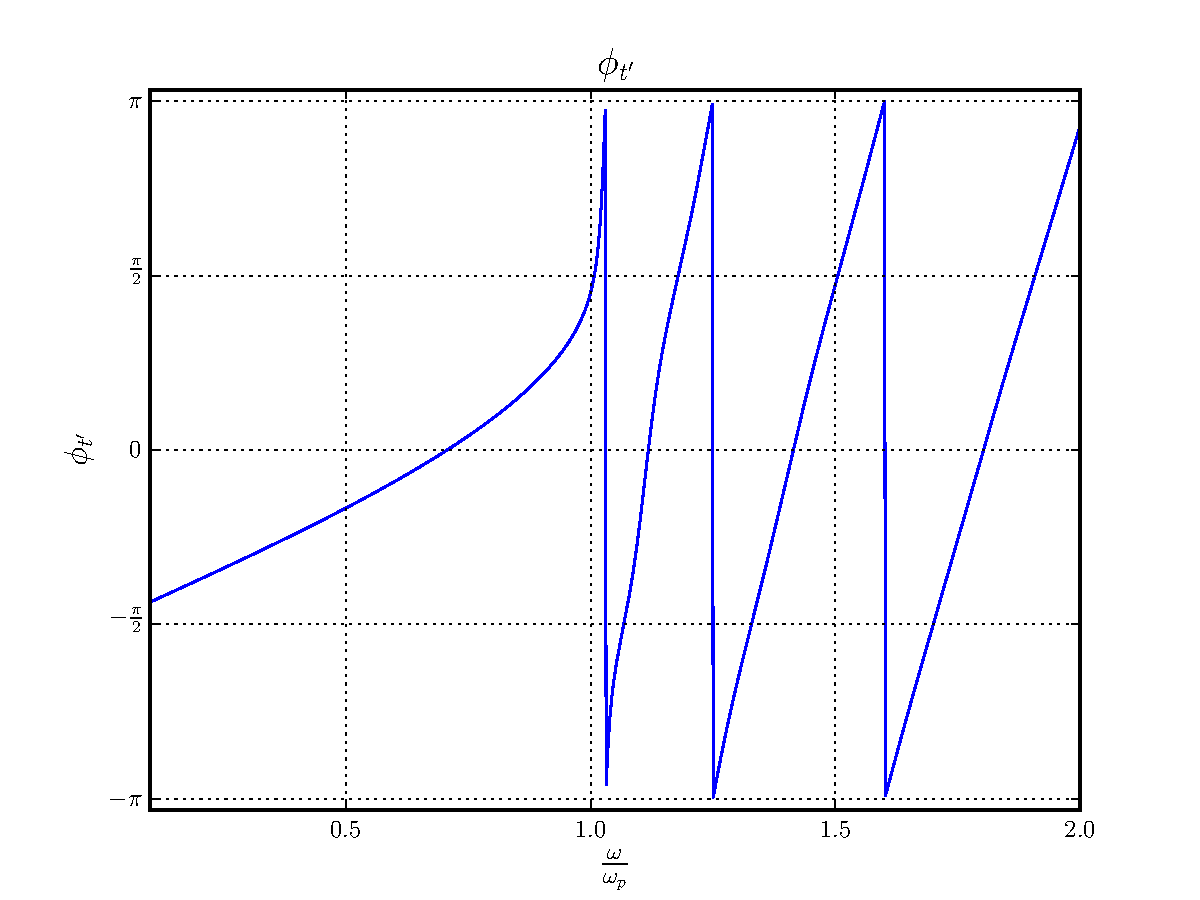
\includegraphics[width=0.9\textwidth]{Punto1BC/tp_f.pdf}
                            \end{figure}
                            %FIGURA

\subsection*{1.d}
                            %FIGURA
                            \begin{figure}[!ht]
                            \centering 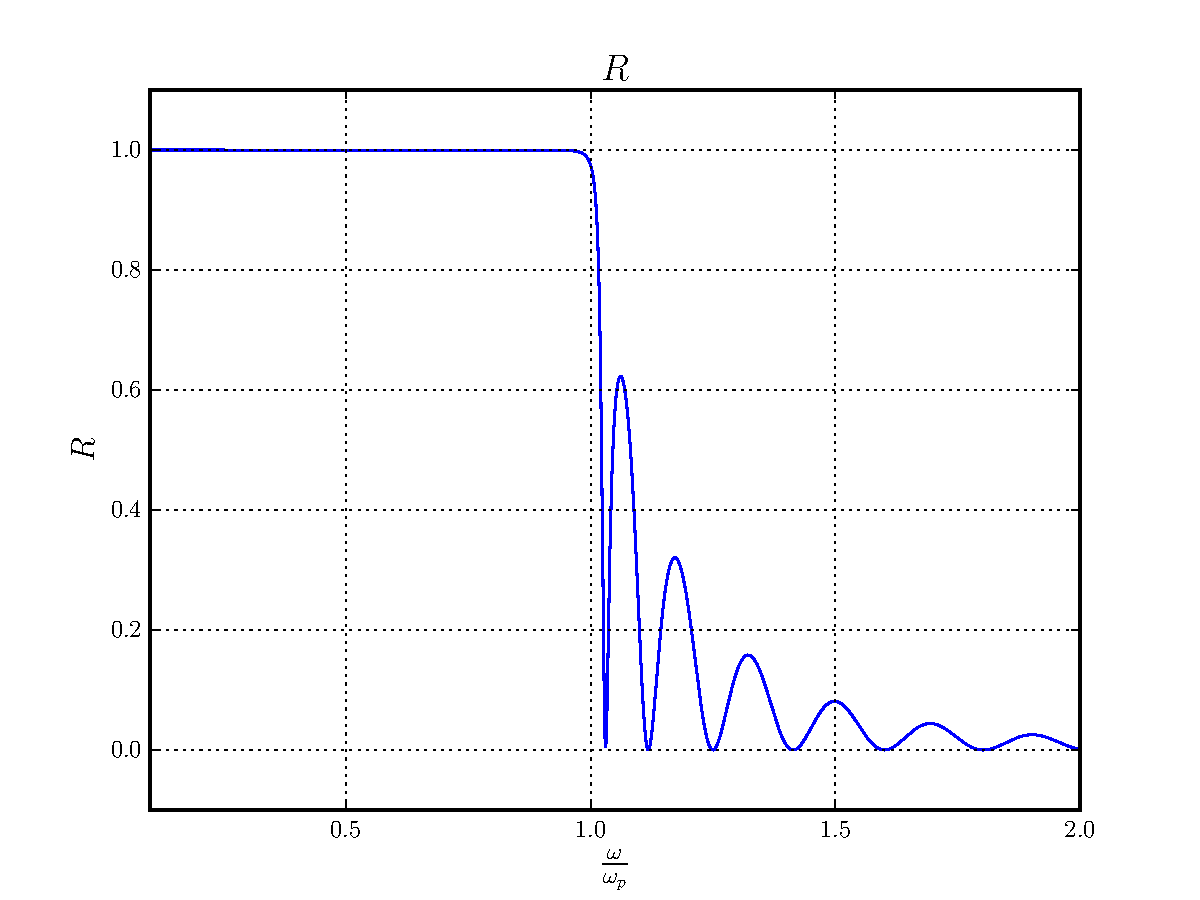
\includegraphics[width=0.9\textwidth]{Punto1BC/R.pdf}
                            \end{figure}
                            %FIGURA
                            %FIGURA
                            \begin{figure}[!ht]
                            \centering 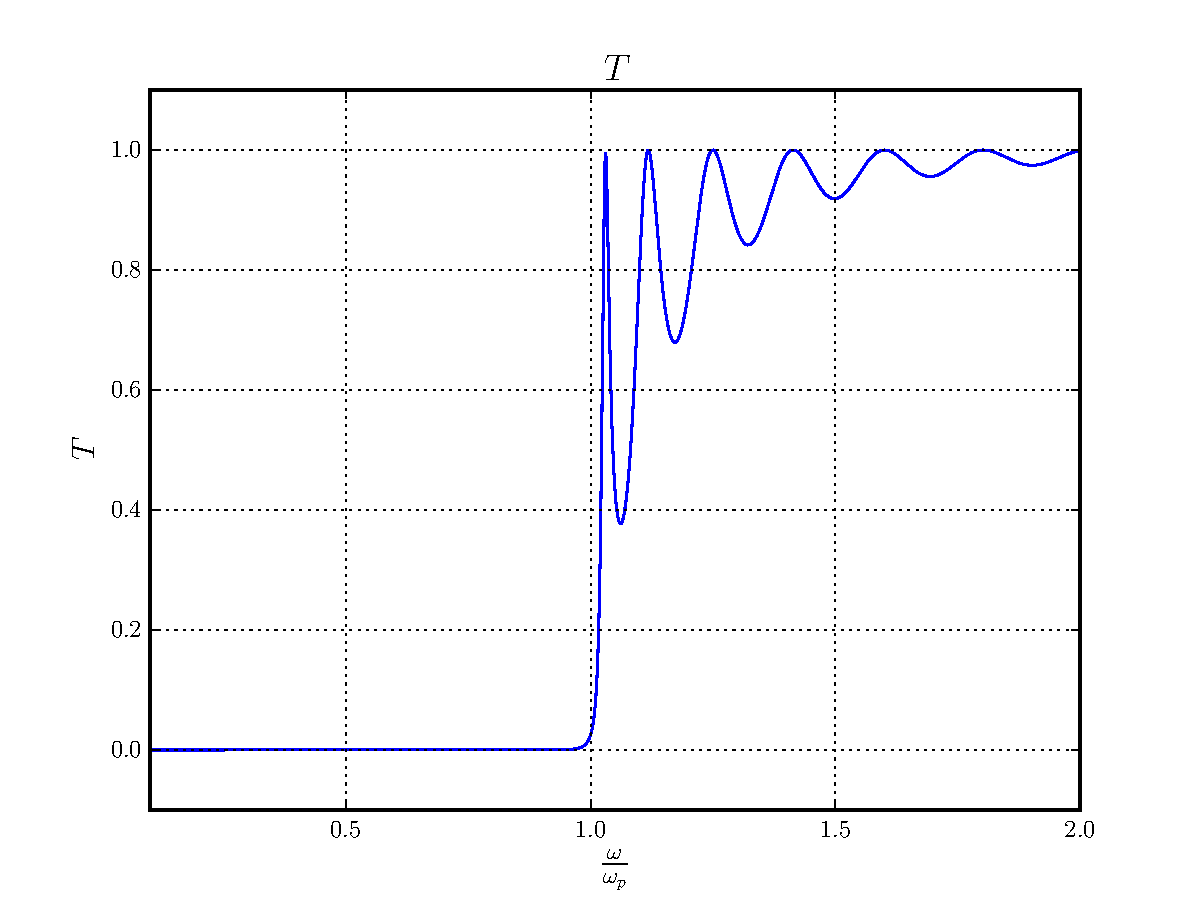
\includegraphics[width=0.9\textwidth]{Punto1BC/T.pdf}
                            \end{figure}
                            %FIGURA


                            %FIGURA
                            \begin{figure}[!ht]
                            \centering 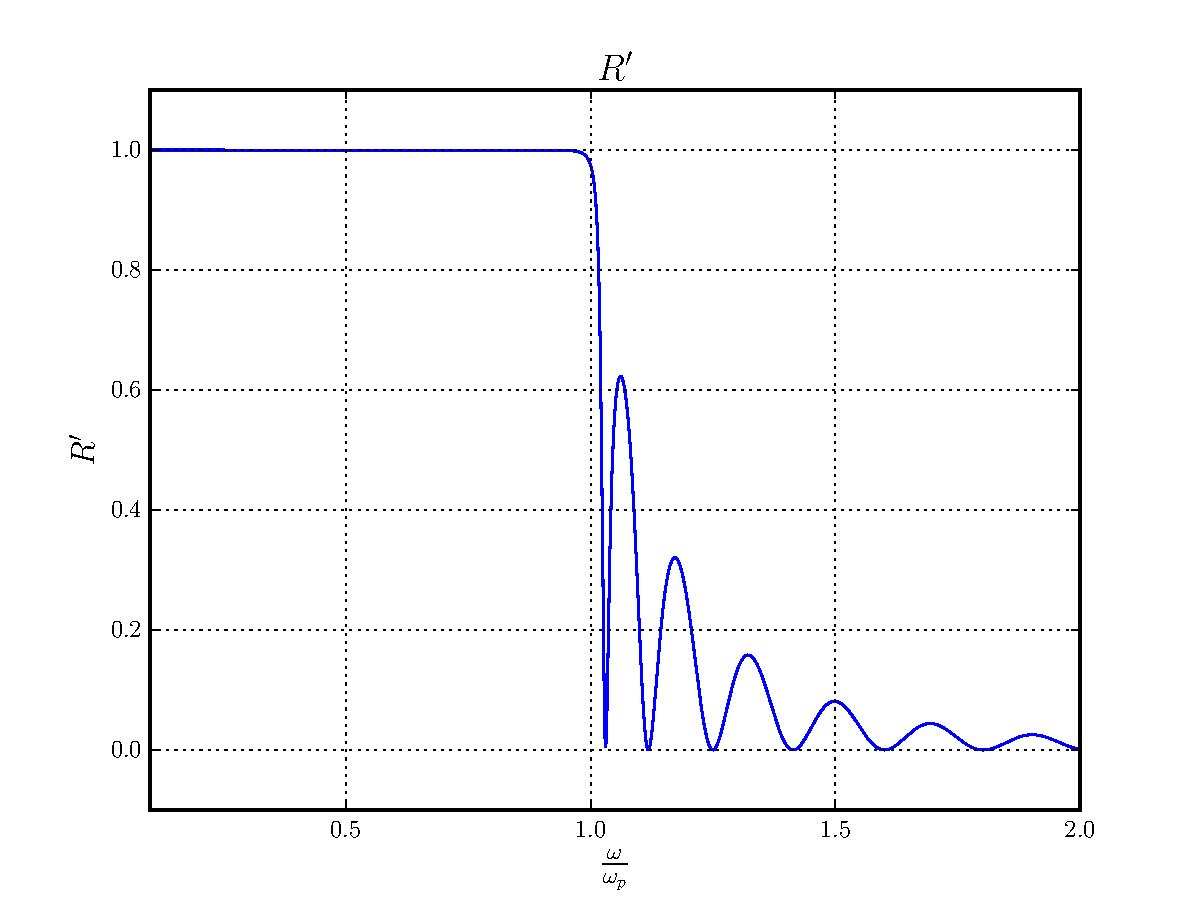
\includegraphics[width=0.9\textwidth]{Punto1BC/Rp.pdf}
                            \end{figure}
                            %FIGURA
                            %FIGURA
                            \begin{figure}[!ht]
                            \centering 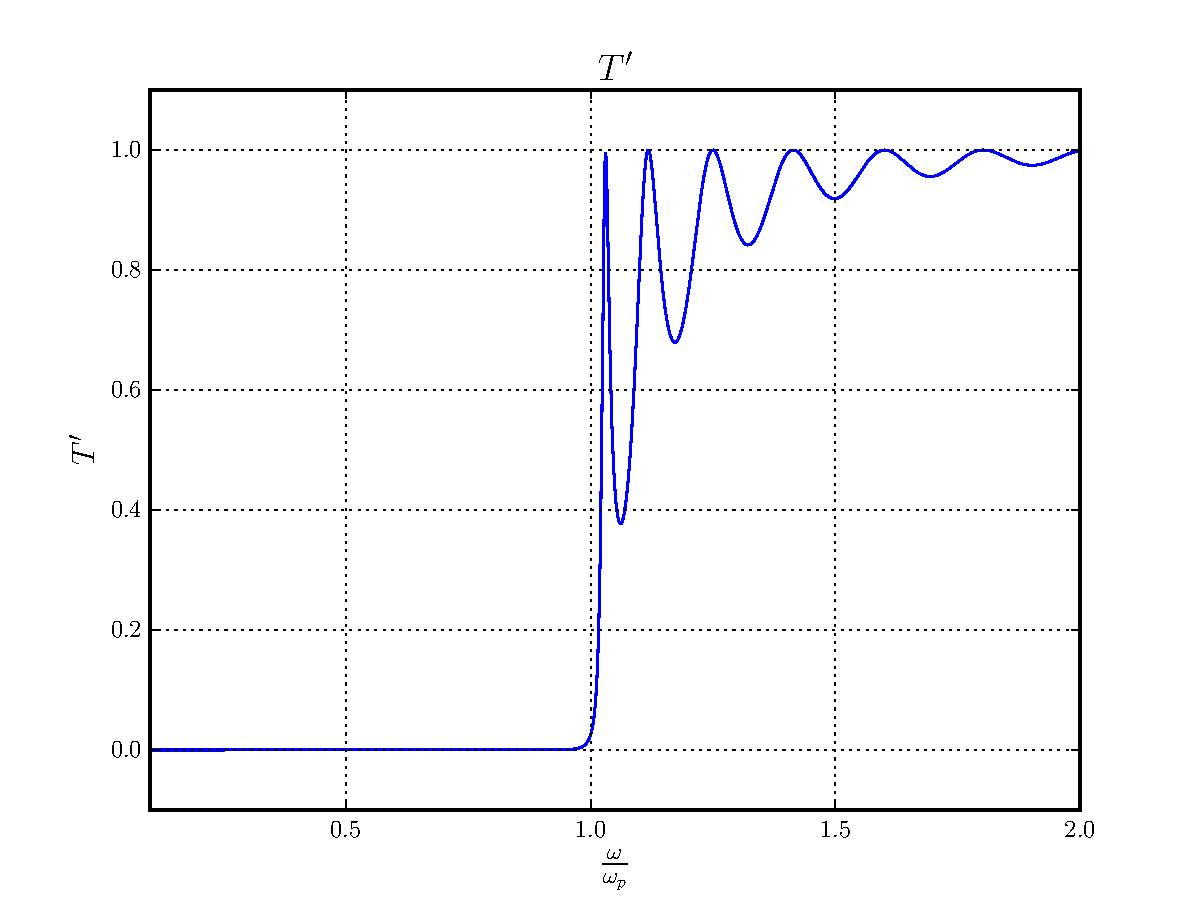
\includegraphics[width=0.9\textwidth]{Punto1BC/Tp.pdf}
                            \end{figure}
                            %FIGURA
Confirmación de $R+T=1$

                            %FIGURA
                            \begin{figure}[!ht]
                            \centering 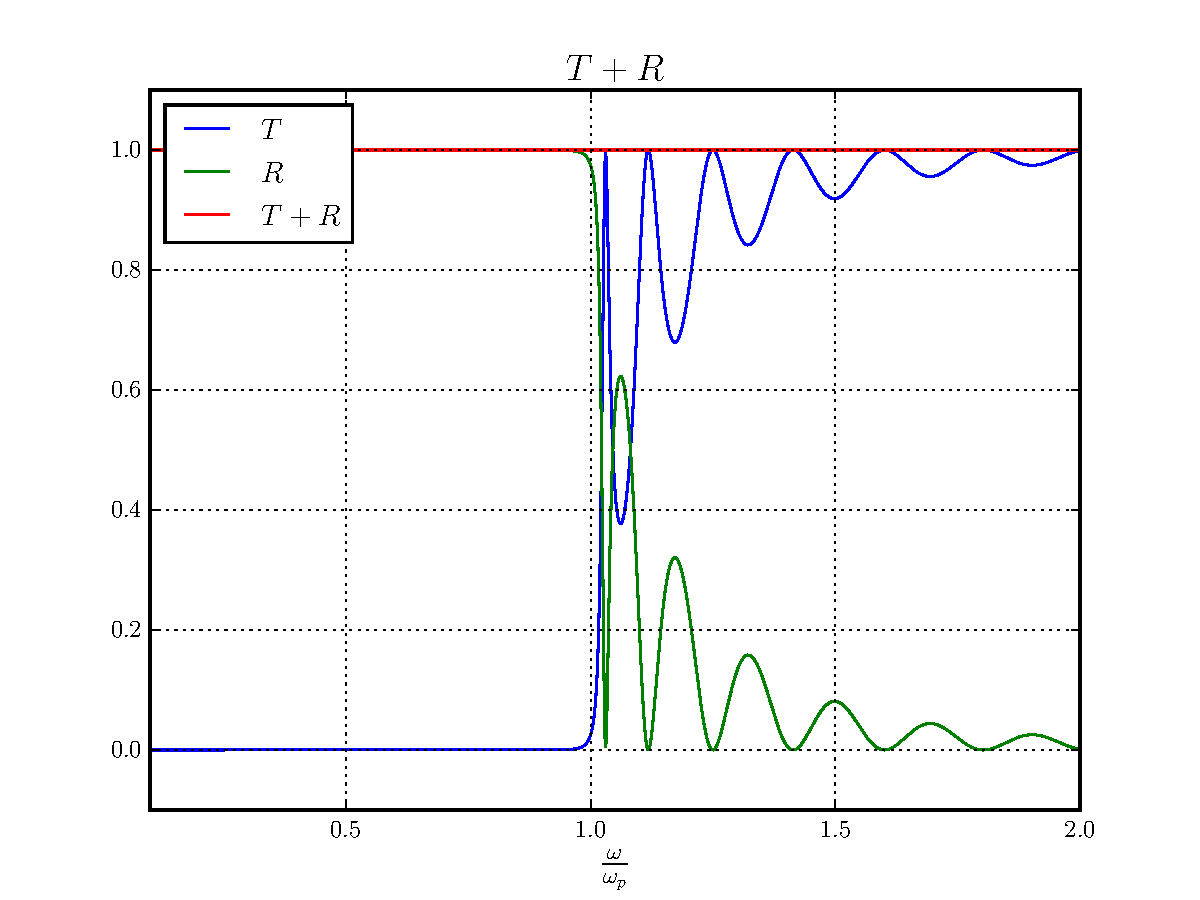
\includegraphics[width=0.9\textwidth]{Punto1BC/RT.pdf}
                            \end{figure}
                            %FIGURA
                            
                            %FIGURA
                            \begin{figure}[!ht]
                            \centering 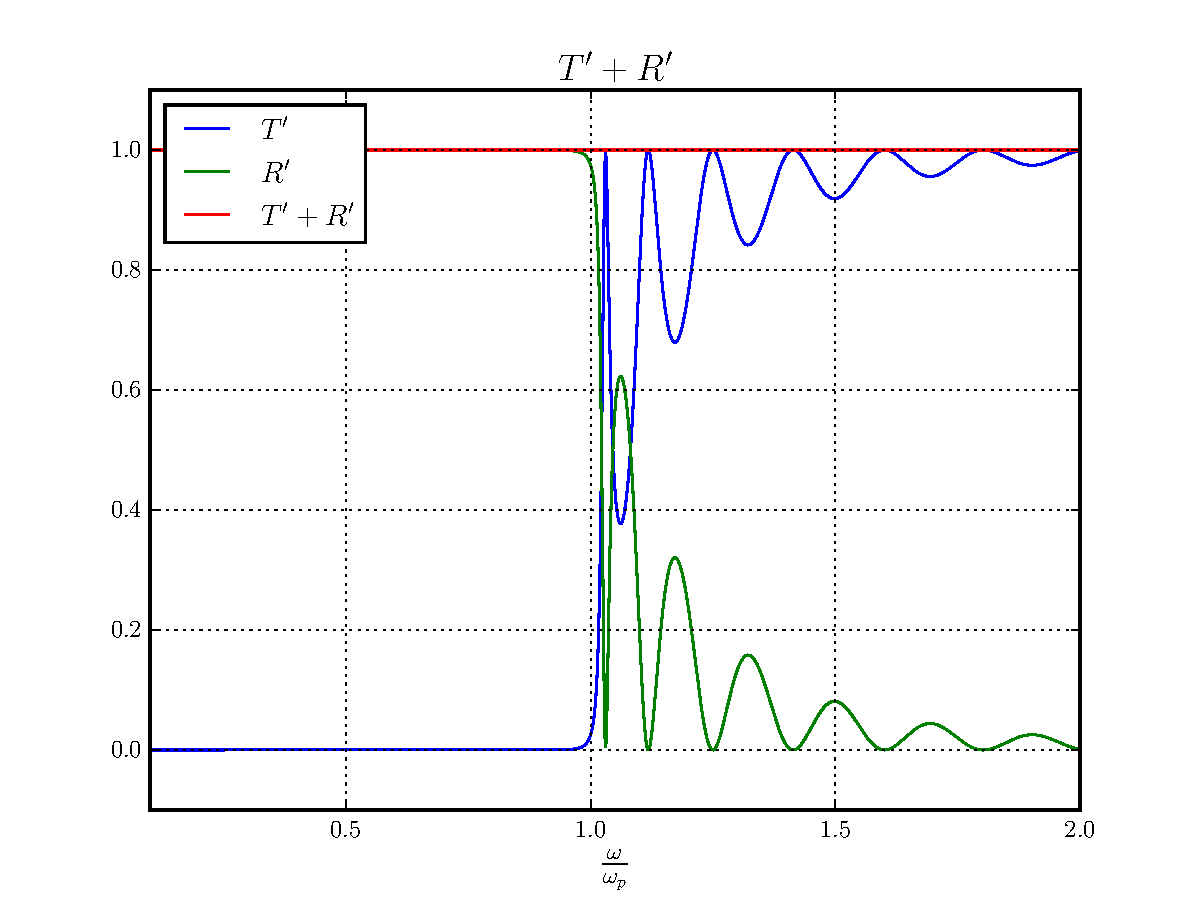
\includegraphics[width=0.9\textwidth]{Punto1BC/RTp.pdf}
                            \end{figure}
                            %FIGURA



\section*{Punto 2}
\subsection*{2.a}
\subsection*{2.b}
\subsection*{2.c}  
\subsection*{2.d}

\section*{Punto 3}
\subsection*{3.a}
\subsection*{3.b}
\subsection*{3.c}  
\subsection*{3.d}

\end{document}
